\documentclass[11pt, letterpaper]{article}
\usepackage{palatino}
\usepackage{graphicx}
\usepackage{enumitem}
\usepackage[top=1in, left=1in, right=1in, bottom=1in]{geometry}

\begin{document}
\begin{center}
\Large{\textbf{Capstone 2 - Model Metrics}}

\large{Kirsten Regier}
\end{center}

\section{Decision Tree Model}
\subsection{Hyperparameters}
\begin{figure}[h]
\begin{center}
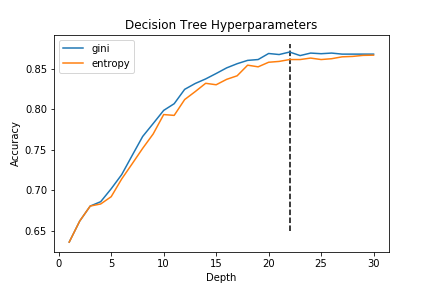
\includegraphics[width=3in]{DTHyperparameters.png}
\caption{Grid search results for \textbf{depth} and \textbf{node purity} method hyperparameters.} 
\label{fig:DTHyper}
\end{center}
\end{figure}

\subsection{Model parameters}
\noindent \textbf{DecisionTreeClassifier}(ccp\textunderscore alpha=0.0, class\textunderscore weight=None, criterion='entropy', max\textunderscore depth=24, \newline max\textunderscore features=None, max\textunderscore leaf\textunderscore nodes=None, min\textunderscore impurity\textunderscore decrease=0.0, min\textunderscore impurity\textunderscore split=None, min\textunderscore samples\textunderscore leaf=1, min\textunderscore samples\textunderscore split=2, min\textunderscore weight\textunderscore fraction\textunderscore leaf=0.0, presort='deprecated', random\textunderscore state=21, splitter='best')

\begin{figure}[h]
\begin{center}
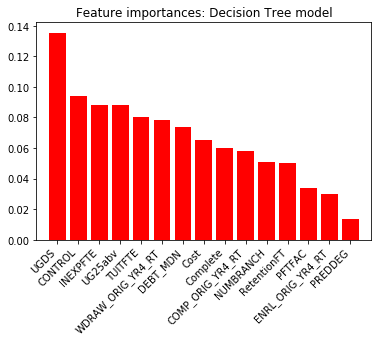
\includegraphics[width=3in]{DTFeatureImportance.png}
\caption{Feature importance levels based on the Decision Tree model.} 
\label{fig:DTFeatures}
\end{center}
\end{figure}

\subsection{Model evaluation}

\begin{table}[h]
\begin{center}
\caption{Decision Tree - Confusion matrix and Evaluation metrics}
\begin{tabular}{l l | c c r }
\multicolumn{2}{l}{Currently operating} & \multicolumn{2}{c}{Predicted} & Recall \\
& & No & Yes &  \\ 
\cline{2-5}
Actual & No & 1525 &  131 & 0.92 \\
& Yes & 302 &1930 & .86 \\  \hline
Precision&  & .83 & .94 \\ 
Accuracy & & &  & .889 \\
\end{tabular}
\label{tab:DTConfusion}
\end{center}
\end{table} 


\section{AdaBoost Model}

\subsection{Hyperparameters}
\begin{figure}[h]
\begin{center}
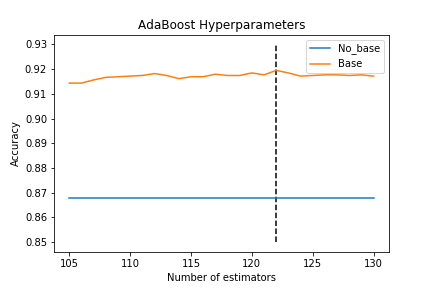
\includegraphics[width=3in]{ABHyperparameters.png}
\caption{Grid search results for \textbf{number of estimators} hyperparameter.} 
\label{fig:ABHyper}
\end{center}
\end{figure}

\subsection{Model parameters}
\noindent \textbf{AdaBoostClassifier}(algorithm='SAMME.R',
                   base\textunderscore estimator=DecisionTreeClassifier(ccp\textunderscore alpha=0.0,
                                                         class\textunderscore weight=None,
                                                         criterion='entropy',
                                                         max\textunderscore depth=24,
                                                         max\textunderscore features=None,
                                                         max\textunderscore leaf\textunderscore nodes=None,
                                                         min\textunderscore impurity\textunderscore decrease=0.0,
                                                         min\textunderscore impurity\textunderscore split=None,
                                                         min\textunderscore samples\textunderscore leaf=1,
                                                         min\textunderscore samples\textunderscore split=2,
                                                         min\textunderscore weight\textunderscore fraction\textunderscore leaf=0.0,
                                                         presort='deprecated',
                                                         random\textunderscore state=21,
                                                         splitter='best'),
                   learning\textunderscore rate=1.0, n\textunderscore estimators=114, random\textunderscore state=21)

\begin{figure}[h]
\begin{center}
%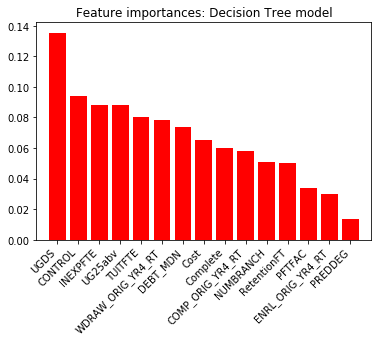
\includegraphics[width=3in]{DTFeatureImportance.png}
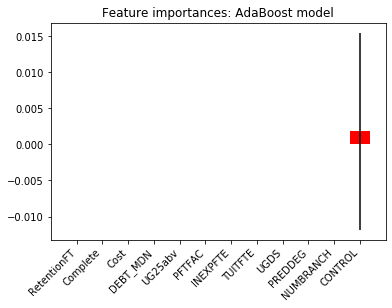
\includegraphics[width=3in]{ABFeatureImportance.png}

\caption{Feature importance levels based on the AdaBoost model.} 
\label{fig:Features}
\end{center}
\end{figure}

\subsection{Model evaluation}

\begin{table}[h]
\begin{center}
	\caption{AdaBoost Model - Confusion matrix and Evaluation metrics}
		\begin{tabular}{l l | c c r }
\multicolumn{2}{l}{Currently operating} & \multicolumn{2}{c}{Predicted} & Recall \\
& & No & Yes &  \\ 
\cline{2-5}
Actual & No & 1536 &  120 & 0.93 \\
& Yes & 171 & 2061 & .92 \\  \hline
Precision&  & .90 & .94 \\ 
Accuracy & & &  & .93 \\
	\end{tabular}
	\label{tab:ABConfusion}
	\end{center}
	\end{table}

\end{document}